%
% Projekt: simulation_study.tex
% Autor:   Michal Ľaš
% Datum:   03.12.2023
%


\documentclass[a4paper, 11pt, a4paper]{article}
\usepackage[left=2cm,text={17cm, 24cm},top=3cm]{geometry}

\usepackage[slovak, english]{babel}
\usepackage{times}
\usepackage{color}
\usepackage[utf8]{inputenc}
\usepackage[T1]{fontenc}
\usepackage[hidelinks]{hyperref}
\usepackage{url}
\usepackage{graphicx}
%\usepackage[colorinlistoftodos,prependcaption,textsize=tiny, disable]{todonotes}

% Images folder
\graphicspath{{../images/}}

% TODO command
\newcommand{\todo}[1]{\textcolor{red}{\textbf{[[#1]]}}}



\begin{document}

% Title page
\begin{titlepage}
    \begin{center}
            \textsc{\Huge Brno University of Technology \\}
            \vspace{0.5em}
            \textsc{\huge Faculty of Information Technology \\}
        \vspace{\stretch{0.382}}
            {\LARGE 	Modelling and Simulation\,--\,Project (T5: SHO Model of logistics) \\
            \vspace{0.4em}
            \Huge The use of electric and autonomous cars in the transport company Packeta}
        \vspace{\stretch{0.618}}
    \end{center}
    {\Large \today \hfill Michal Ľaš (xlasmi00), Adam Lazík (xlazik00)}
\end{titlepage}

% Table of contents
\tableofcontents
\newpage

% Body
\section{Introduction}

The objective of this project is to formulate a model [\cite{IMS.lectures}, slide 7] for the logistics, transport, and parcel delivery operations of Packeta,
a company specializing in these services. The primary aim of this model [\cite{IMS.lectures}, slide 7] is to determine the optimal ratio of conventional, electric,
and autonomous vehicles for practical implementation in last-mile delivery. Concurrently, the simulation [\cite{IMS.lectures}, slide 8] experiments are designed to
explain the financial implications associated with employing different modes of transport and to assess efficiency under varying loads,
measured by the number of parcels for delivery.

To achieve these goals, a specific depot within the Žilina region was selected for the study, namely, the Žilina, Strečno depot.


\subsection{Study sources}

The primary source of resources for this project was derived from the official website of Packeta \cite{packeta}.
Due to the company's reluctance to disclose internal information beyond what is officially published,
supplementary data essential for model creation was gathered from articles \cite{delivery.distance}, \cite{delivery.percentage},
\cite{parcels.num}, the internet \cite{peugeot}, and professional papers.
Notably, information about autonomous cars was predominantly sourced from scientific articles \cite{autonomous.emissions}, \cite{autonomous.models}.


\subsection{Model validation}

% validity [\cite{IMS.lectures},  slide 37]
\noindent\todo{Ako sa nám podarilo overiť validitu modelu}


\subsection{Used technologies and procedures}

The implementation of the project utilized the C++ programming language along with the SIMLIB library \cite{SIMLIB}.
These technologies were chosen for their suitability in addressing the specified problem, offering a requisite interface,
ease of use, and being freely accessible.


\section{Facts and Hypotheses}

The factual basis for the project primarily relied on information about the vehicles used by Packeta, sourced from the official
website of the vehicle manufacturer. The number of parcels a courier can deliver daily was derived from article \cite{parcels.num} on the internet,
featuring the CEO of Packeta, who highlighted the effectiveness of parcel lockers and address deliveries. According to the article,
a courier can deliver approximately 100 parcels to an address and up to 2500 parcels per day to parcel lockers. This information was
cross-referenced with data on the popularity of various delivery destinations \cite{delivery.percentage} to calculate the average number of
parcels that the courier can deliver per day.

The model also incorporates the cost of courier services, a factor considered due to its elimination with autonomous cars.
The price of courier work was obtained from job portals and the official website of Packeta, where such job details are available.

The characteristics of autonomous cars were chosen hypothetically, drawing from articles \cite{autonomous.emissions} and \cite{autonomous.models}. These values were adjusted with a
forward-looking perspective, aiming for a greater range and capacity to enhance their significance for a company like Packeta. The delivery
time for autonomous cars was determined hypothetically, considering the optimization of traffic navigation, an advantage inherent in sophisticated
control systems.

Average delivery distances were determined based on the delivery locations map available on Packeta's official website \cite{packeta} and the geographical
structure of the Žilina region. Specifically, areas in the north of Slovakia were identified as being 65\,--\,75 kilometers away from the
distribution depot (Žilina, Strečno). The circular route of an electric delivery vehicle covering such distances could pose challenges,
particularly in the winter months when the range of electric cars tends to decrease.


\section{Model Design}

Parcels are delivered from the designated depot daily and they are categorized into two distinct groups. The initial group contains parcels
necessitating delivery beyond the operational range of electric or autonomous vehicles, constituting 2\,--\,8\% \cite{packeta} of the entire parcel volume.
The average distance covered for deliveries in this group spans 180\,--\,200 kilometers \cite{packeta}. The fuel cost for the vehicle employed by the designated
company is 1,705€ per liter, with a fuel consumption rate of 8.8 liters per 100 kilometers \cite{peugeot}.

The second group, constituting 98\,--\,92\% \cite{packeta} of the parcels, encompasses those amenable to delivery through all available means. The average distance
covered for deliveries in this category ranges from 130\,--\,150 kilometers \cite{packeta}, \cite{delivery.distance}. Each courier is equipped to handle 1274\,--\,1574 parcels \cite{parcels.num}, \cite{delivery.percentage}, inclusive of loading,
transportation, and unloading, within their 8-hour work shift. Couriers utilizing electric cars recharge their vehicles overnight at the depot, ensuring
they are ready for the next day's deliveries. The cost of electricity is approximately 0.185€ per kilowatt-hour (kWh), and the electric car in use has a
consumption rate of 0.35 kWh per 100 kilometers \cite{peugeot}.

Upon completion of their work hours, couriers leave and return the subsequent day. The courier's salary, ranging from 1600\,--\,2000€ per day, is counted into
the daily operational costs for both electric and conventional vehicles. Autonomous vehicles exclusively rely on electricity and require charging.
Nevertheless, they are capable of delivering parcels throughout the day. If some parcels destined for the address or the pick-up place are not delivered in time, their delivery is moved to the next day.
It is assumed that during the night, autonomous vehicles either
charge or deliver parcels to designated parcel lockers. Consequently, parcels destined for pick-up places and specific addresses receive priority.
The preference for delivery destinations is distributed as follows: 44\% for direct delivery to addresses, 35\% for delivery to pick-up places,
and 21\% for the favored option of delivery to parcel lockers \cite{delivery.percentage}.

An autonomous car possesses an average transport capacity of 400\,--\,600 parcels per battery charge, and the average delivery time for parcels ranges
from 2 to 6 hours. The charging time is 30 minutes and during this time the car can also be loaded with packages for delivery. This loading takes 30-60
minutes. An autonomus car in use has a consumption rate of 0.25 kWh of electricity per 100 kilometers \cite{autonomous.emissions}.

Model created with Petri net [\cite{IMS.lectures}, 126] is in figure \ref{figure:scheme}.

\begin{figure}[ht]
    \begin{center}
        \scalebox{0.6}{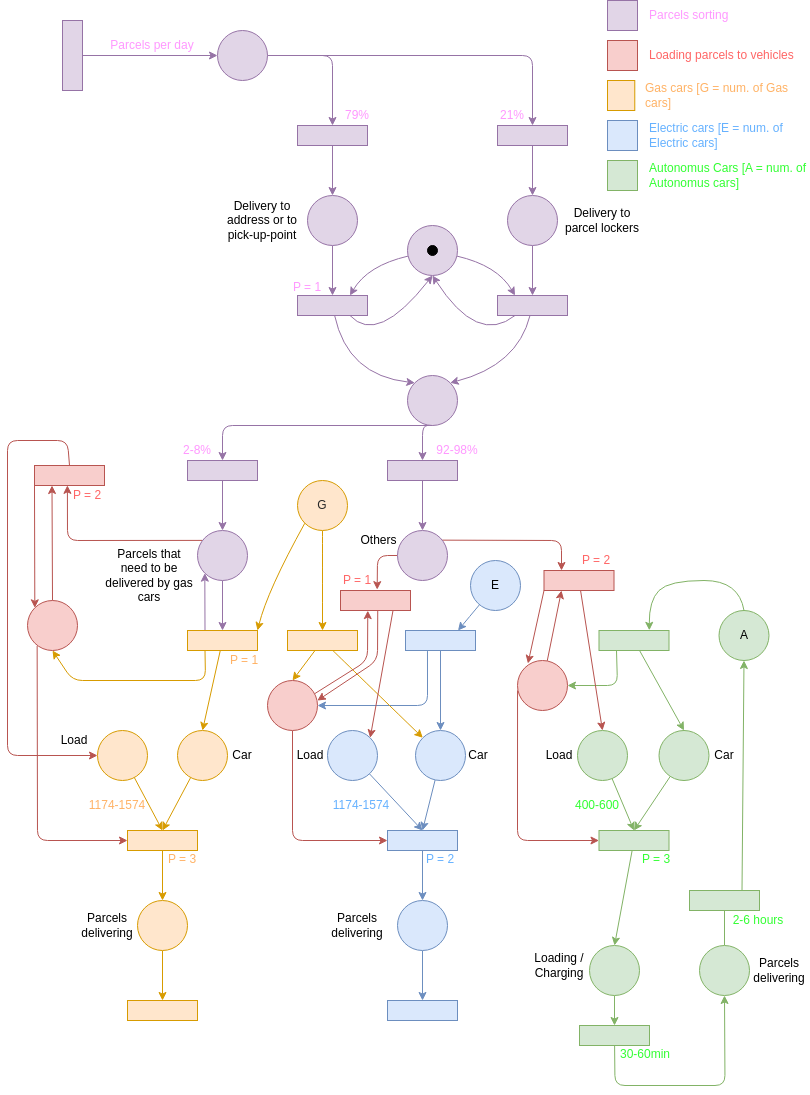
\includegraphics{../images/scheme.png}}
    \end{center}
    \caption{Petri net [\cite{IMS.lectures}, 126] model}
    \label{figure:scheme}
\end{figure}


\section{Architecture of the simulation model}

Model is implemented as class \texttt{WorkDay} and the simulation is started by running
\texttt{./main} with the following arguments:
\begin{itemize}
    \item \texttt{-d DAYS} - number of days. Each day is
    an individual simulation executed with the arguments below (except parcels remaining from the previous day, we
    will get to it later).
    \item \texttt{-p PARCELS} - number of parcels to run simulation with
    \item \texttt{-g GAS\_CARS} - number of gas cars to run simulation with
    \item \texttt{-g ELECTRIC\_CARS} - number of electric cars to run simulation with
    \item \texttt{-g AUTONOMOUS\_CARS} - number of autonomous cars to run simulation with
\end{itemize}
To learn more about arguments, run \texttt{./main -h}.

\newpage

\noindent Work day lasts 24 hours from 8:00 to 8:00 on the following day.
At the beginning, parcels are sorted to four categories:
\begin{itemize}
    \item parcels to distant address or pick-up point
    \item parcels to near address or pick-up point
    \item parcels to distant Zbox (parcel locker)
    \item parcels to near Zbox (parcel locker)
\end{itemize}
Implementation-wise there is no difference between parcels to pick-up point and
addresses, hence they are grouped together.
Parcels are then loaded into available cars based on the order specified in the
model.
Parcels to distant location take priority as they can only be loaded into gas
cars.
Parcels to addresses or pick-up points are loaded before parcels to Zboxes as
they into the queue first based on the model.
The car cannot be loaded if the parcel batch would not reach the maximum
capacity. The maximum size of the batch
is generated from uniform distribution as packages differ in size.

The driver of electric car or gas car ends his shift after delivering all the
packages in his car and driving the car back to the depot. It is presumed that
the driver manages to do this within working hours, so there is no need to
measure time on those types of cars.

While the work day has not ended and autonomous cars could still be loaded, the
model waits for an autonomous car to return. If the car returns and time
remaining to the end of the work day is greater or equal to maximum possible
operation time of the autonomous car (maximum loading time + maximum delivery
time), the car is loaded with another parcel batch (although implemented
as a new autonomous car object). Autonomous cars cannot deliver packages to
addresses or pick-up points after 18:00 as this is the end of regular human work
day. \newline

\noindent At the end of the work day, the following statistics are collected and printed
out:
\begin{itemize}
    \item parcels shipped
    \item parcels remaining
    \item gas car operation cost
    \item electric car operation cost
    \item autonomous car operation cost
    \item total operation cost
\end{itemize}
Operation cost includes price of the consumed fuel and driver's daily salary
(missing in autonomous cars). Both are generated from uniform distribution based
on values acquired by research mentioned in the previous sections.

If there are any parcels remaining, they are added to the parcels generated on
the next day.

\section{Experiments}

\todo{Pipis vykonaných experimentov, ich dôvod, výsledky a zistenia}


\section{Conclusion}

\todo{Čo sa nám podarilo experimentami dokázať}


% Literature
\newpage

\bibliographystyle{enplain.bst}
\renewcommand{\refname}{Sources}
\bibliography{simulation_study}

\end{document}
